%! Author = Gabriela
%! Date = 07.01.2023

\documentclass[]{article}
\usepackage[utf8]{inputenc}
\usepackage[T1]{fontenc}
\usepackage{ragged2e}
\usepackage{geometry}
\usepackage{graphicx}
\graphicspath{ {./images/} }
\geometry{a4paper, margin=1in}

\title{
    
\includegraphics[]{header.png} \\
    Projektowanie i integracja systemów (PIS) \\
    \bigskip MAGAZYN \\
    \begin{center}
        
\includegraphics[]{logopw.png}
    \end{center}
}
\author{
    Daniel Kobiałka\\
    daniel.kobialka.stud@pw.edu.pl \\
    310744 \\
    \and
    Bartłomiej Dudek\\
    bartlomiej.dudek.stud@pw.edu.pl \\
    310623 \\
    \and
    Adam Sudoł\\
    adam.sudol.stud@pw.edu.pl \\
    310933 \\
    \and
    Karol Rogoziński\\
    karol.rogozinski.stud@pw.edu.pl \\
    310883\\
    \and
    Gabriela Topczewska \\
    gabriela.topczewska.stud@pw.edu.pl \\
    310961 \\
}
\date{09.01.2023}

\renewcommand{\contentsname}{Spis treści}

\begin{document}

    \maketitle

    \newpage
    \tableofcontents{}

    \newpage
    \section{Postawiony problem}
    \subsection{Pomysł}
    Pomysł na projekt zrodził się z zapotrzebowania osób trzecich na program służący do obsługi magazynów. Opis problemu został dostarczony drogą mailową i załączony jest poniżej:

    \begin{center}
        \textit{Jest plac, który stanowi powierzchnie magazynową. Powierzchnia podzielona jest na jakieś mniejsze powierzchnie które stanowią sektory. Każdy sektor ma jakiś tam metraż powierzchni w m2. Każdy sektor to powierzchnia na której składamy palety z pustakiem ceramicznym. Pustak występuje w sumie w 25-30 rodzajach. Są dwa rodzaje palet jeśli chodzi o rozmiar 120/100 cm i 136/100. Niektóre z wyrobów piętruje się na 3 do góry, niektóre na 4 warstwy. Są tez jakieś drobnicowe materiały. \\  (...) Od poniedziałku do piątku 7-17 są prowadzone załadunki samochodów paletami z pustakiem z tegoż magazynu, jednocześnie 7 dni w tygodniu 24h idzie produkcja, i wyroby z tej produkcji są składowane na magazyn. Każdy kierowca przyjeżdżając na załadunek rejestruje się w terminalu samoobsługowym, gdzie dostaje dokument dostawy w którym jest opisane min co dokładnie ma mieć załadowane. \\  (...) Operator wózka podejmując kolejne auto do załadunku widzi na tablecie oprócz jakiś podstawowych danych czyli nr rejestracyjny auta, nazwisko kierowcy, widzi również co dokładnie ma załadować na to auto, a co najważniejsze widzi skąd ma to załadować, czyli np. 5 palet PTH25E3 z sektora B3 i 15 palet PTH 11,5 z sektora D8. Pobierając te palety z wyznaczonych miejsc potwierdza iż załadunek co jednocześnie powoduje iż w danych sektorach stan magazynu zostaje zmniejszony o wydana ilość i rodzaj. Jednocześnie inny wózkowy w tym samym czasie prowadząc wywóz palet z produkcji odstawia te palety w konkretny wcześniej wyznaczony przez koordynatora magazynu sektor. \\ Założenie jest takie , żeby na bieżąco było widać gdzie mamy ile zmagazynowane jakiego asortymentu, ile mamy powierzchni wolnej, ile w danym sektorze przy zapełnieniu np. w 30 \% zmieści mi się jeszcze palet itp. Żeby można było zaplanować kolejność w jakiej poszczególne sektory/ asortyment będzie wydawany do klienta lub też zapełniony z produkcji. }
    \end{center}
    \bigskip
    \subsection{Główne funkcjonalności}
    Po analizie problemu sformułowano i wyznaczono główne funkcjonalności aplikacji:
    \begin{enumerate}
        \item definiowanie magazynów i ich podsekcji, w tym ich wymiarów,
        \item przypisywanie podsekcjom konkretnych produktów,
        \item zarządzenie kontami użytkowników,
        \item tworzenie i zarządzenie zleceniami przez kierownika,
        \item przeglądanie historii zleceń dla danej sekcji lub magazynu,
        \item przeglądanie przez pracownika przypisanych mu zleceń
        \item generowanie raportów o stanie magazynu.
    \end{enumerate}

    \section{Proponowana implementacja}
    W ramach projektu zaproponowano dostarczenie aplikację webową z backendem pisanym w języku Java, frontendem z użyciem biblioteki Spring i relacyjną bazą danych na serwerze MySQL. \\
    Proponowana implementacja umożliwia łatwy dostęp do aplikacji z dowolnego urządzenia (laptop, tablet, telefon komókowy), co stanowi ważny element postawionego zadania.

    \section{Stos technologiczny}
    Poniżej przedstawiono spis narzędzi i technologii używanych w projekcie:
    \begin{itemize}
        \item Java 2137,
        \item SpringBoot,
        \item React
        \item Maven,
        \item Git,
        \item GitHub,
        \item MySQL,
        \item Aplikacje ELK:
        \begin{itemize}
            \item ElasticSearch,
            \item Logstash,
        \end{itemize}
        \item JUnit,
        \item DataJpaTest,
        \item PDFBox,
        \item JDBC,
        \item IDE: IntelliJ Idea
        \item maszyny wirtualne Azure
        \item dokumentacja: LaTeX
    \end{itemize}

    \section{Organizacja pracy}
    W celu organizacji pracy zdecydowano się używać portalu Discord jako głównego narzędzia komunikacyjnego. Serwer dostosowano do potrzeb projektu:

    \begin{center}
        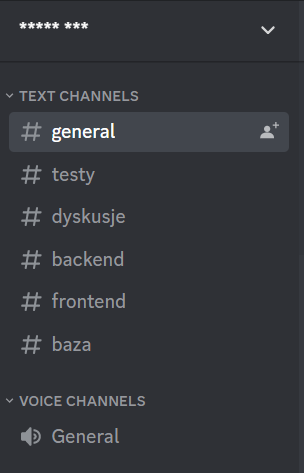
\includegraphics[scale=0.8]{discord.PNG}
    \end{center}

    Oprócz Discorda do komunikacji używano komunikatora Messenger, kontaktu telefonicznego oraz spotkań na żywo. Komunikacja z mentorem zespołu przebiegała głównie drogą mailową. \\
    Stan prac i ich postęp kntrolowany był za pomocą narzędzi oraz opcji dostępnych w ramach serwisu GitHub oraz narzędzia Git.

    \section{Baza danych}

    \subsection{Serwer}
    Serwerem bazodanowym, którego użyto w projekcie jest serwer MySQL. Został on postawiony na maszynie wirtualnej Azure z systemem Ubuntu. Aby podnieść poziom bezpieczeństwa i jakości dostrczonego rozwiązania skonfigurowano replikę bazy, działającą na innej maszynie dostępnej przez portal Azure. \\
    \begin{center}
        
\includegraphics[scale=0.05]{MySQL-Logo.png}
    \end{center}

    \subsection{Diagram ER}
    Poniżej zaprezentowano diagram relacyjny stworzonej bazy:

    \begin{center}
        
\includegraphics[scale=0.8]{sql.PNG}
    \end{center}

    Jak widać powyzej, w bazie znajdują się następujące tabele:
    \begin{enumerate}
        \item Magazyny
        \item Sekcje
        \item Produkty
        \item Pracownicy
        \item Zlecenia
        \item Raporty
    \end{enumerate}

    Struktura magazynu opisanego w bazie danych jest następująca:

    \bigskip
    Magazyn podzielony jest na sekcje, w których znajdują się określone produkty (w każdej z sekcji jeden produkt). Zarówno magazyn jak i sekcja mają swoje wymiary określone w metrach. Dodatkowo, sekcja posiada współrzędne jednego z wierzchołków tak, aby można było jednoznacznie wyznaczyć jej obszar na mapie magazynu.

    \bigskip
    Pracownicy magazynu dzielą się na kierownikó oraz pozostałych pracowników. Kierownicy mogą wystawiać innym pracownikom zlecenia, w których określają co należy wykonać.

    \bigskip
    Kierownicy magazynu mogą generować raporty PDF opisujące aktualny stan magazynu. Raporty te, oprócz pobierania na maszynę użytkownika wysyłane są też do bazy danych, gdzie są przechowywane.

    \subsection{Dokładne charakterystyki tabel}
    \subsubsection{Magazyny}
    Tabela \textit{Magazyny} posiada następujące atrybuty:
    \begin{enumerate}
        \item \textit{id} - id magazynu,
        \item \textit{name} - nazwa magazynu,
        \item \textit{length} - długość magazynu w metrach,
        \item \textit{width} - szerokość magazynu w metrach,
    \end{enumerate}

    \subsubsection{Sekcje}
    Tabela \textit{Sekcje} posiada następujące atrybuty:
    \begin{enumerate}
        \item \textit{id} - id sekcji,
        \item \textit{magazyn\_id} - id magazynu, w którym znajduje się dana sekcja,
        \item \textit{produkt\_id} - id produktu przechowywanego w danej sekcji,
        \item \textit{name} - nazwa sekcji,
        \item \textit{amount} - liczba sztuk produktu w sekcji,
        \item \textit{length} - długość sekcji w metrach,
        \item \textit{width} - szerokość sekcji w metrach,
        \item \textit{bottom\_left\_point\_x} - X-owa współrzędna lewego dolnego rogu sekcji,
        \item \textit{bottom\_left\_point\_y} - Y-owa współrzędna lewego dolnego rogu sekcji.
    \end{enumerate}

    \subsubsection{Produkty}
    Tabela \textit{Produkty} posiada następujące atrybuty:
    \begin{enumerate}
        \item \textit{id} - id produktu,
        \item \textit{name} - nazwa produktu,
        \item \textit{length} - długość magazynu w metrach,
        \item \textit{width} - szerokość magazynu w metrach,
        \item \textit{stack\_size} - liczba palet z produktem, które mogą być na siebie nałożone.
    \end{enumerate}


    \subsubsection{Pracownicy}
    Tabela \textit{Pracownicy} posiada następujące atrybuty:
    \begin{enumerate}
        \item \textit{id} - id pracownika,
        \item \textit{first\_name} - imię,
        \item \textit{last\_name} - nazwisko,
        \item \textit{login} - login w aplikacji,
        \item \textit{password\_hash} - hash hasła do konta w aplikacji,
        \item \textit{is\_manager} - oznaczenie, czy pracownik pełni rolę kierownika.
    \end{enumerate}


    \subsubsection{Zlecenia}
    Tabela \textit{Zlecenia} posiada następujące atrybuty:
    \begin{enumerate}
        \item \textit{id} - id zlecenia,
        \item \textit{name} - tytuł,
        \item \textit{description} - treść zlecenia,
        \item \textit{kier\_id} - id kierownika wystawiającego zlecenie,
        \item \textit{prac\_id} -id pracownika, który ma wykonać zlecenie,
        \item \textit{status} - status wykonania zlecenia.
    \end{enumerate}


    \subsubsection{Raporty}
    Tabela \textit{Raporty} posiada następujące atrybuty:
    \begin{enumerate}
        \item \textit{id} - id raportu,
        \item \textit{file} - treść raportu w postaci BLOBa.
    \end{enumerate}



    \section{Backend}
    \subsection{ELK Stack}
    W celu wykorzystania możliwości przeszukiwania pełnotekstowego w aplikacji wykorzystano narzędzia dostarczane przez ELK Stack. Skorzystano z możliwości hostowania serwisów w chmurze Elastic Cloud.

    \begin{center}
        
\includegraphics[scale=0.4]{elk-stack-logo.png}
    \end{center}

    \subsubsection{ElasticSearch}
    W chmurowej wersji ElasticSearchu przechowywana jest kopia danych z MySQLowej bazy w postaci indeksów i dokumentów. Dzięki temu możliwe jest skorzystanie z funkcjonalności oferowanej przez ElasticSearch. \\
    Dla każdej tabeli z bazy relacyjnej istnieje odpowiadający jej indeks, w którym trzymane są dokumenty z rekordami. W szczególności istnieje indeks raportów, dzięki czemu generowane pliki PDF również mogą być przeszukiwane. \\ Funkcją która w tym projekcie jest szczególnie przydatna, jest wyszukiwanie dopuszczające popełnianie literówek.

    \bigskip
    Dane logowania do portalu ElasticSearch umieszczone zostały w pliku \textbf{application.properties}.

    \subsubsection{Logstash}
    Dane pomiędzy bazą MySQL, a ElasticSearchem synchronizowane są za pomocą aplikacji Logstash. Napisany został skrypt konfiguracyjny, dzięki któremu z użyciem interfejsu JDBC dane z MySQLa są pobierane i wysyłane do odpowiadających im indeksów w ElasticSearchu. Z powodów technicznych skrypt Logstasha uruchamiany jest raz na jakiś czas, a dane aktualizowane są wsadowo (zob. sekcja \textit{10. Napotkane problemy i ich rozwiązania}).

    \section{Frontend}

    \section{Testy}

    \section{Uruchomienie aplikacji}

    \section{Napotkane problemy i ich rozwiązania}
    Podczas tworzenia aplikacji napotkano następujące problemy:
    \begin{itemize}
        \item \textbf{Zbyt mało wydajne maszyny wirtualne dostępne w ramach portalu Azure} - podczas konfigurowania narzędzi z ELK Stack początkowo przyjętą taktyką było skonfigurowanie ich w Dockerze w sieci utworzonej na maszynach wirtualnych. Niestety okazało się, że zasoby wybranych maszyn wirtualnych są niewystarczające, by te dały radę hostować serwisy i umożliwiać ciągłą synchronizację bazy MySQL z jej dokumentową kopią w ElasticSearchu. Zmiana maszyn nie była dostępną opcją, ze względu na fundusze dostępne w ramach licencji studenckiej Azure. Z tego powodu przyjętym rozwiązaniem stało się hostowanie ElasticStacka w chmurze, a synchronizacja danych przeprowadzana zostaje wsadowo z urządzenia jednego z członków projektu, posiadającego dostęp do serwera MySQL za pomocą skryptów Logstasha i interfejsu JDBC.
    \end{itemize}
    \section{Wnioski końcowe}

\end{document}